\chapter{Evaluation\label{chap3}}

For the system to be successfully utilized within the project
it needs to accomplish the following goals:
\begin{enumerate}
\item It needs to be able to integrate the daily tasks of the users
      without it being a burden.
\item It needs to effectively  manage the data items and
      coordinate the tasks between the users and the system.
\end{enumerate}

In order to answer these questions, the system needed to be evaluated on two
fronts. \emph{User Experience} evaluations were performed to test whether the
system could be easily adopted by users if implemented.

The system was then tested further to see if it could perform
a subset of the tasks it would be required to perform if implemented within
the \emph{Zamani Project}. Due to time constraints, the entire set of tasks required
to support the activities of the Zamani Project could not be implemented.

\section{User Experience Evaluation}
Users and their experience of a system is becoming a critical component
in designing a software system\cite{Forlizzi:2004:UEI:1013115.1013152}.

User Experience evaluations aim to understand the needs and experiences of a user.
In order to do this, user engagement needs to be tested on both a visual and emotional level.
These evaluations are used to link the needs of the users to the functionality provided by the
system. The benefit gained from having a usable system is that the productivity
of the users is greatly increased\cite{nielsen2003usability}.
User Experience experiments were performed to ensure that the system
provides a good, usable interface.

\subsection{Aim}
The aim of the usability test is to assess the quality of the system. This
assesses the user's ability to complete required tasks efficiently while
remaining satisfied with the system\cite{bevan1995measuring}. This is done in
order to determine how suitable the solution is for the user.

The usability of the system was be rated using the following attributes
\cite{doi:10.1207/s15327590ijhc1803_3}:
\begin{description}
\item[Learnability] Relates to the capability of the software to enable a user
    to learn how to use it. This is a goal for the system as this would
    enable users to quickly start using the software effectively.
\item[Efficiency] Refers to the time it takes for the
    user to complete a certain goal or task.
\item[Satisfaction] Measures the attitude of the users towards software. This
    includes: \begin{inparaenum}[(i)]\item Difficulty;\item Confidence; and
        \item Like/Dislike towards the system\end{inparaenum}.

\item[Error] Number of errors that a user makes, including deviations from
    the intended path.
\item[Effectiveness] This tests user efficiency based on a predetermined level
    in terms of speed, number of errors and steps.
\item[Simplicity] Amount of effort that is required for a user to complete a
    task. This can be traced in terms of number of selections or time taken to
    search for a function.
\end{description}

To measure the user experience, a simple performance evaluation is not
enough. We need to be able to gain insight on how users feel about the system
\cite{vermeeren2010user}. This requires that the emotional state of the user be
evaluated.

\subsection{Methodology}
In order to determine the attributes mentioned above, a quantitative \emph{User Experience}
 experiment was set up. Users were asked to complete two task using
the system. The system was designed to support a workflow. This involves two main
user activities: \begin{inparaenum}[(i)] \item Management of individual tasks;
and \item Setting up workflows \end{inparaenum}. The tasks were designed to test
these operations. Their experiences were recorded and then evaluated. The detailed
process is outlined below.

\subsubsection{Task Setup}
Tasks were set up for users to complete. The aim of these tasks was to simulate
the main activities of the system. This led to the formalisation of two tasks
that are described as follows:
\begin{description}
\item[Complete a set of tasks as a user] \hfill \\
    The first part was to simulate the actions of an unprivileged user
    who is required to do outstanding tasks.  A Site was created containing three
    tasks. These tasks were assigned to the test user. Since the system aims to
    support tasks that are executed on the user's workstation, the tasks were
    designed to be as simple as possible. Since the general usability of the system
    was to be evaluated, the tasks were not related to processing digital cultural
    artifacts.

    Three \emph{Python} programs were set up to represent the user tasks
    that were to be executed. For \emph{Task one} and \emph{Task two},
    the user was simply required to run the desktop application. The third
    task, however, aims to test the user's understanding of the system by
    asking the user questions about the task. These questions are:
    \begin{inparaenum}[(a)] \item What is the output directory for the
    task?;  and \item Please select the input files that are used in this
    task\end{inparaenum}?   The task descriptions all convey what the purposes
    of the tasks are. As soon as the user completes a task, they need to
    indicate on the system that the task has been completed.
\item[Build a simple workflow] \hfill \\
    For the second part the user had to simulate the role of a privileged
    user, and had to set up a sample workflow. The tasks represent a workflow
    that produces a PDF file starting with a text file. This was given as a
    diagram to the users. The diagram can be seen in Figure~\ref{eval:workflow}.
        The user was given very little instruction on how to complete the task.
    This allows them to explore the system and intuitively complete the task.

\end{description}
\begin{figure}[!h]
    \begin{center}
        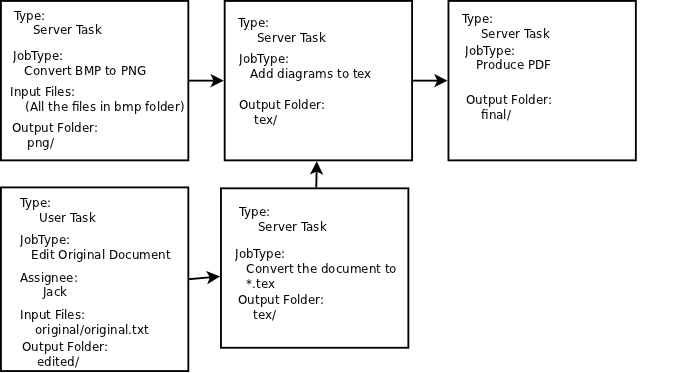
\includegraphics[scale=0.45]{figures/workflow.png}
    \end{center}
    \caption{Workflow that needed to be recreated}
    \label{eval:workflow}
\end{figure}
To ensure that each user experienced the system the same way, it was restored to
its previous state after each test.

\subsubsection{Questionnaire}
The primary method used to evaluate the \emph{User Experience} of the system was
using a questionnaire. Questionnaires attempt
to obtain the subjective feelings of the user towards the
system\cite{Chin:1988:DIM:57167.57203}. In order to measure the experience, the
emotional response of the user also has to be obtained. The USE questionnaire
was chosen to evaluate the User Experience \cite{lund2001measuring}. This
questionnaire is designed to determine the usability attributes in terms of:
\begin{inparaenum}[(i)]\item Usefulness;\item Ease of Use; \item Ease of learning; and \item
Satisfaction \end{inparaenum}. It is designed in such a way that an
emotional response is triggered. In order to avoid \emph{Acquiescence Response Bias},
the questionnaire duplicates responses in such a way that the they were
phrased both negatively and positively.
In order to save on paper, the survey was conducted using \emph{Lime
Survey}\footnote{Lime Survey: http://www.limesurvey.org/},
The questionnaire used can be found in Appendix~\ref{appendix:questionnaire}.

\subsubsection{Monitoring and Pilot Tests}
During the tests the users were monitored and their actions noted. This was to
determine what the overall process was for each of the users. All
questions, actions and errors were also noted during this process. These events
were noted by time to produce the remaining usability attributes namely:
\begin{inparaenum}[(i)]\item Efficiency; \item Error; \item Effectiveness; and \item
Simplicity  \end{inparaenum}

After the tasks were set up, the user tests were run using two users. This was
used to determine problems that would adversely affect the results before it was
run using a larger test group. The results of the pilot test identified some
minor issues regarding how the questions were worded, that distracted the users
from the task at hand. This was fixed before the full tests were conducted.

\subsubsection{User Selection}
The participants chosen for the user experiment were not the users that would
be interacting with the system on a daily basis. This is to avoid confirmation
bias that is likely to occur due to the fact that they are stakeholders in the
project\cite{kaptchuk2003effect}. 

The participants varied in age ranging from 18 to 24. Due to cost and time
constraints all subjects tested were students. The level of
technical competence varied from novice to expert. The students were highly
diverse in terms of \emph{Field of Study}, being drawn from four faculties:
Economics, Engineering, Science, and Humanities. 24 participants were used 
to perform the evaluation.

\subsection{Results}
The user evaluation produced a number of results. Users were on average able to
finish the task $21$ minutes, with an interquartile width of
$7$ minutes. This indicates that the users were mostly able to complete the task
in the expected time. All but one of the users were able to complete the
entire set of tasks that were provided. Results of the test were acquired using two
methods: the survey; and the data from the observations.

The survey independently measured data for both tasks that the participants were
required to execute. This aimed to get the users' opinions on the categories
regarding: \begin{inparaenum}[(i)] \item Usefulness; \item Ease of use; \item
Ease of Learning; and \item Satisfaction \end{inparaenum}. Values with a high
amount of variance were not considered to be significant.\\

\subsubsection{Execute Simple Tasks}
The participants were asked to evaluate their experiences with regard to
completing the tasks. The survey, along with the observations was used to
rate the experience in terms of the following categories:
\begin{description}
    \item[Usefulness] \hfill \\
    	Overall, the users found that the system was useful and allowed them to be
    	productive. There is a general indication that the system was well
    	equipped to support the tasks that were executed by the participants.
	$76\%$ of participants found the system useful.

    	From observation it seemed that users were easily able to use the system
    	to indicate the tasks. There appeared to be very little confusion as to
    	what the purpose of the buttons on the interface was.

    	There was a slight delay, for about $30\%$ of users, between the
	completion of the first task and
    	when the users started the second task since the task screen displayed
    	either that \emph{data was being transferred back} or that the task
    	was \emph{awaiting validation}. They seemed to wait for the system to
    	indicate that the status has changed, without realising that the
    	validation process was manual. This reduced the initial usefulness of
    	the system, prompting that more interactive task reporting is possibly
    	required.
    \item[Ease of use] \hfill \\
    	The number of steps required to complete the task was considered to be
    	minimal by $80\%$ of the users, and very few inconsistencies were
	noted. $71\%$ of participants agreed that the system was easy
	and simple to
    	use. The system was described as flexible and users were able to
    	recover from mistakes easily.

    	It should be noted that participants initially found the concept of
    	specifying \emph{input files} and the \emph{output folder} while
    	completing \emph{Task $3$} confusing. $50\%$ of users had to be told
    	what the task was asking. From the user responses, this can likely be
    	attributed to phrasing of \emph{Task $3$} within the system.

    \item[Ease of Learning] \hfill \\
        The system was described as being very easy to learn by  $90\%$ of
    	participants. They found that the system was very easy to remember.
    	$75\%$ of users described themselves as somewhat skilful after using
	it for a short	period of time.

    	This corresponds with the observations made during the test. Since
    	participants were given no instructions on how to use the system, they
    	were initially quite hesitant to perform actions. However, as the
    	experiment moved along, their actions became much faster and more
    	decisive.

     \item[Satisfaction] \hfill \\
        $85\%$ of participants were satisfied with the experience
	with the system and that it allowed
        them to complete the tasks with relative ease. Users emotionally
        responded to the system in the following way: \begin{inparaenum}[(i)]
    	\item it was pleasant to use; and \item that the system was
        wonderful\end{inparaenum}.

        Some users showed clear signs of satisfaction when they started getting
        used to the interface. At no point did any of the participants appear
        frustrated while completing the first part of the experiment.

    \item[Efficiency] \hfill \\
        The efficiency of the survey was not measured by the survey and all
        findings are based on the observations of the users. Users took an
        average time of $7$ minutes in completing the first task. The slowest
        time taken was $12$ minutes. The interquartile range was determined
        to be between $5$ minutes and $8$ minutes, showing that most of the
        users were able to efficiently accomplish the tasks provided.

        Some efficiency issues were noted in the hesitance of participants
        after completing the first task, before starting the second task.
        This could be attributed to the participants being unfamiliar with the
        system; however it is an indication that better task feedback would
        likely increase efficiency.
\end{description}
Overall, the task interface yielded positive results on the \emph{User
Experience} of the system. Layout issues were identified that caused users
to navigate to unexpected places, but users were quickly able to recover from
this without needing assistance. The learnability tests showed that the system
was very easy to learn and it required very little effort on the part of the
participants to use it successfully.

\subsubsection{Build Simple Workflow\label{eval:simple}}
For this task the participants were asked to build a simple workflow, that had
been provided on a diagram. (See Figure~\ref{eval:workflow}) The instructions
did not provide any information on how the system should be used and
participants were required to determine how to complete the task on their own.
\begin{description}
\item[Usefulness] \hfill \\
    $85\%$ of participants indicated that they found the system to be
    effective for the task that was required. $80\%$ also indicated that
    the system aided them in being productive and completing the task.
    Overall, $94\%$ of users found the system useful.

    Users found that the system gave them good control over what they were doing and
    made the task relatively easy to complete, and felt the number of steps
    involved were appropriate.

    Observations of the participants revealed that the participants quickly
    understood what was expected and were able to use the system to
    effectively build the workflow that was required. All users were able to
    complete the task.
\item[Ease of Use] \hfill \\
    $85\%$ of participants indicated that they found the system simple and easy to use.
    They believed that the number of steps were minimal to complete the tasks
    that were required. Inconsistencies within the system was not noted by
    the participants. $75\%$ of users felt like they were easily able to recover after
    making an error. They were confident that the system was being used
    successfully. In addition, $75\%$ of users commented very favourably on
    ease of use.

    While monitoring the user interaction, users navigated the entire page before
    deciding on how they would add a task. Typically they would select the
    \emph{User Task} and be confused that the option for the \emph{Server Task}
    was  not available. Several users were directed to the cancel button. This
    indicates that the option should be combined and indication as to what the
    task type is should appear in the combobox.

    Users did seem to intuitively understand that the tasks could be dragged
    within
    the visualisation. Furthermore, since the creation of a task placed the node
    in a fixed position in the visualisation, users seemed to believe that their previous task
    had been overwritten. Stronger visual cues on the nodes in the visualisation
    should be added to indicate that drag options are available. Nodes should
    also initially be randomly placed to avoid confusion. A similar problem was
    noted in dragging the \emph{arrow icon} to indicate dependencies.

    A rather significant problem was encountered during the testing. While
    the users were navigating the page to determine what to do, they encountered
    the Jobs section, believing this is where they needed to add tasks. This
    wasted a lot of time for some users. This is caused by the confusing
    terminology that was used. Better naming convention should be established to avoid
    this problem.
\item[Ease of Learning] \hfill \\
    Users were very quickly able to determine how the system worked and how to
    use it efficiently. Participants grew much more confident and decisive as
    the task progressed. This is also validated by $85\%$ of the responses in
    the survey, that indicated that the system was very easy learn.
    Participants did not hesitate between tasks and quickly added all the
    required nodes.
\item[Satisfaction] \hfill \\
    $90\%$ of users were very satisfied with the system; and $57\%$ agreed
    that the  system was fun to use.
    Participants felt that the system worked the way
    they expected it to work. Emotional responses, that give a better indication of the user
    experience, indicated that a significant portion of the users believed the
    system to be wonderful and that they need to have it. Overall, $80\%$
    users found
    the system pleasant to use.

    During the experiment, the users were noted to express excitement and
    happiness was expressed when they realised how the system works.


\item[Efficiency] \hfill \\
    Users took an average of $7$ minutes to complete, with an interquartile range
    of $5$ to $9$ minutes. Once the participants had placed the first task, they
    were immediately more efficient. The efficiency of the participants was
    quite varied. Some participants spent a significant amount of time
    staring at the visualisation, as they thought that the previous tasks had
    been removed, due to the \emph{drag-and-drop} functionality not being
    apparent.
\end{description}

\noindent The second task was overall rated as a positive experience; while some participants
expressed the need for more complete instructions, on using
the system. However, based on the data acquired on the \emph{learnability} of the
system, this appears to have been the appropriate choice. The experiment strongly
indicated that the \emph{Job} terminology would need to be reworked. Further
observations showed that more visual cues are required to indicate that the
tasks nodes are \emph{draggable}.

The user study was able to highlight problems associated with the system. These
include: \begin{inparaenum}[(i)]\item Task Feedback; \item Navigation; \item
Visual cues; and \item certain Terminology\end{inparaenum}. In terms of
usability criteria, \emph{Effectiveness} and \emph{Simplicity} could not be
tested due to resource and time constraints. Findings on the usability were as
follows:

\begin{description}
\item[Learnability] Users were very quickly able to get used to the system and
	became competent in completing the tasks.
\item[Efficiency] Participants were able to complete the tasks in the required
	amount of time. This was done intuitively without giving specific
	information on how to use the interface.
\item[Satisfaction] Users indicated that they were satisfied with the system. It
	was also noted that overall the participants were not frustrated with
	the system. Users confidently used the system and did so with ease.
\item[Error] Participants who did make errors were able to recover swiftly
	using the interface. Problems however did arise with the job terminology
	where users were confusing jobs with tasks, causing errors. Some detours
	were also noted where a group of participants were not able to
	intuitively navigate back to the \emph{Task Overview} screen.
\end{description}



\section{System Test}
The system needs to be evaluated in terms of its applicability to successfully 
manage and coordinate the tasks of the Zamani Project.
 Due to time constraints, however, the full set of the tasks within the project
could not be implemented. In order to evaluate its applicability,  two tests were
 performed to test whether the  solution would work. The first test was designed to
determine the general applicability of such a system, by executing a workflow that
is unrelated, while the second test involves implementing small portion of the tasks
of the Zamani Project to determine if if could be successfully implemented.

\subsection{Applicability Tests}
Two test were performed. The first test was to build a simple workflow that
creates a document. The second test builds a workflow that represents a portion
of the process that creates a 3D model from the raw scan.




\subsubsection{Creating Document}
The purpose of this task is to mix user tasks along with server tasks. This
workflow is the same workflow that was used in the user test. A representation
of the workflow can be seen in Figure~\ref{eval:workflow}.
The process involves: a user creating a ``\emph{.txt}'' file. Images are then
converted to a different format. These are then converted to the \LaTeX~format
with the pictures added. The document is then compiled to a \emph{PDF}.

The workflow was successfully able to build the document. The completed workflow
can be seen in Figure~\ref{eval:document}.

\begin{figure}[!h]
    \begin{center}
        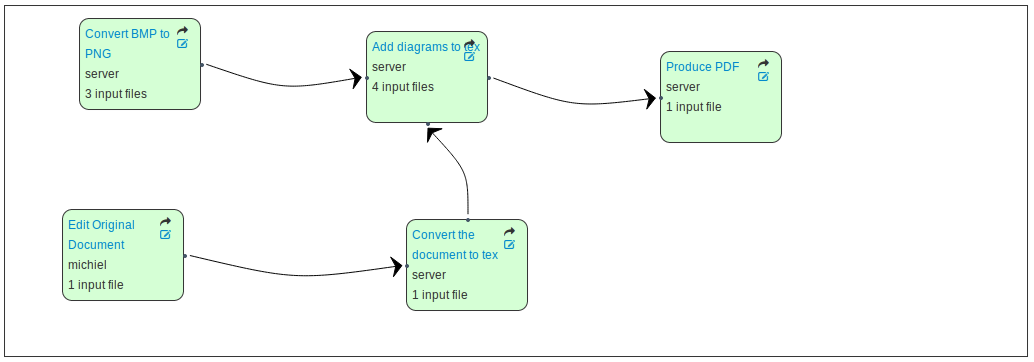
\includegraphics[scale=0.45]{figures/document_test.png}
    \end{center}
    \caption{Completed workflow that creates a simple PDF document}
    \label{eval:document}
\end{figure}

\subsubsection{Integration Test}
A lengthy process is requires to build the 3D models from the initial laser scans require a lengthy
process. This process can be illustrated in Figure~\ref{eval:zamani}
\footnote{Source: Zamani Project at UCT}.
 In order to test whether the system can be applied successfully, a portion of this process
was implemented in the system.

\begin{figure}[!h]
    \begin{center}
        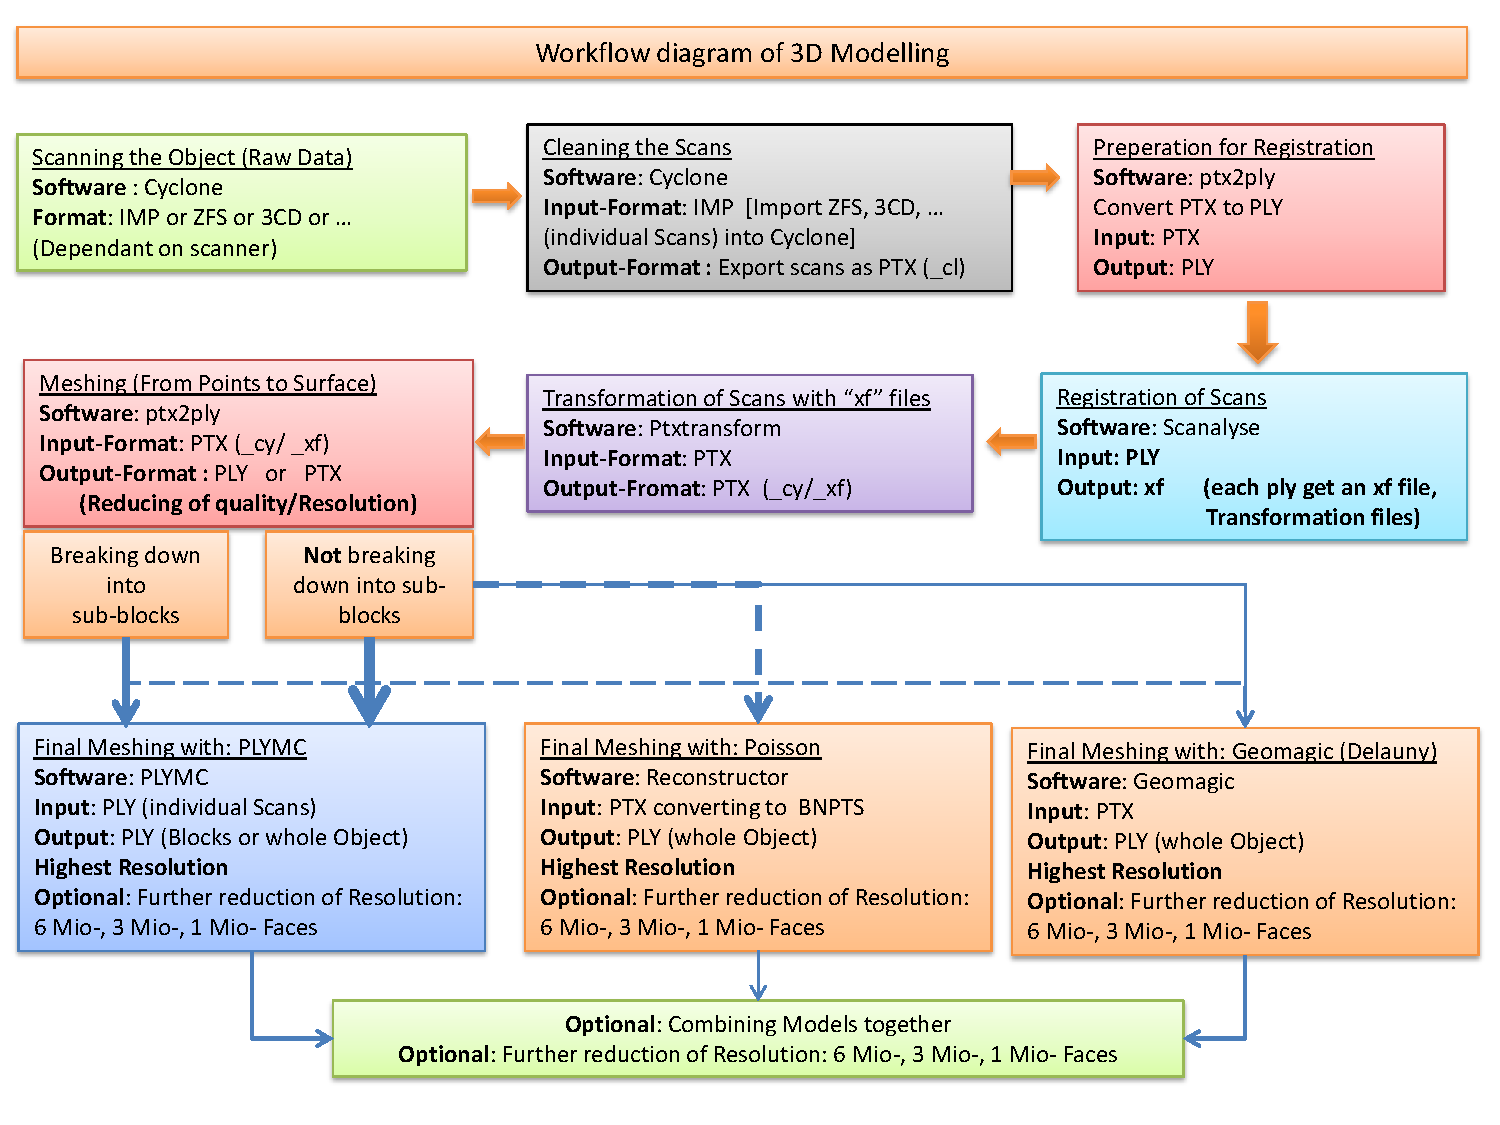
\includegraphics[scale=0.65]{figures/zamani_workflow.pdf}
    \end{center}
    \caption{Zamani - 3D Modelling Workflow}
    \label{eval:zamani}
\end{figure}
The first five steps in the modelling process were implemented using the workflow
system to determine how the system would support running on actual data. Since
data from a previous site was available, the user tasks were merely simulated
by copying over the required data for this task. This was implemented
successfully. Figure~\ref{eval:zamani_impl} shows the workflow being executed.

\begin{figure}[!h]
    \begin{center}
        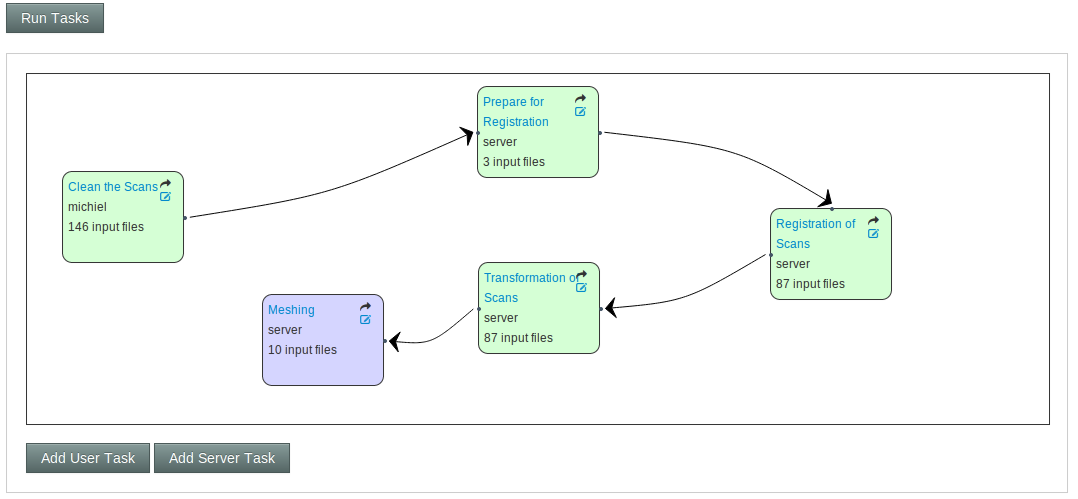
\includegraphics[scale=0.45]{figures/zamani_impl.png}
    \end{center}
    \caption{Partially implemented Zamani modelling workflow}
    \label{eval:zamani_impl}
\end{figure}

\noindent This successful integration shows that the system is able to support some
workflows required by the Zamani project.


\subsection{Filtering}
The system can successfully implement the workflow required for the Zamani
Project, however filtering workflow at a site level is not ideal. Many workflows
get replicated at a building level and beyond this the artifact creation can
also be distinguished by category. In order for the workflows built within the
system to be more reusable, it would need to be extended to store workflows at
finer level. These could then be nested in a hierarchical manner. This would
allow entire workflows to be abstracted as a single node. This would decrease
set up time and increase reusability of the system, however, further
experimentation would be required to determine the effect on User Experience.

\subsection{Performance}
The movement and processing of data is regarded as being the most expensive
portion of the process. The data movement is directly offloaded to \emph{rsync},
whereas the data processing is offloaded to the native applications. The system
management of these activities outperforms these tasks. As such, the system's
performance is bounded by these activities. This offloading procedure is
illustrated in Figure~\ref{eval:offload}.

\begin{figure}[!h]
    \begin{center}
        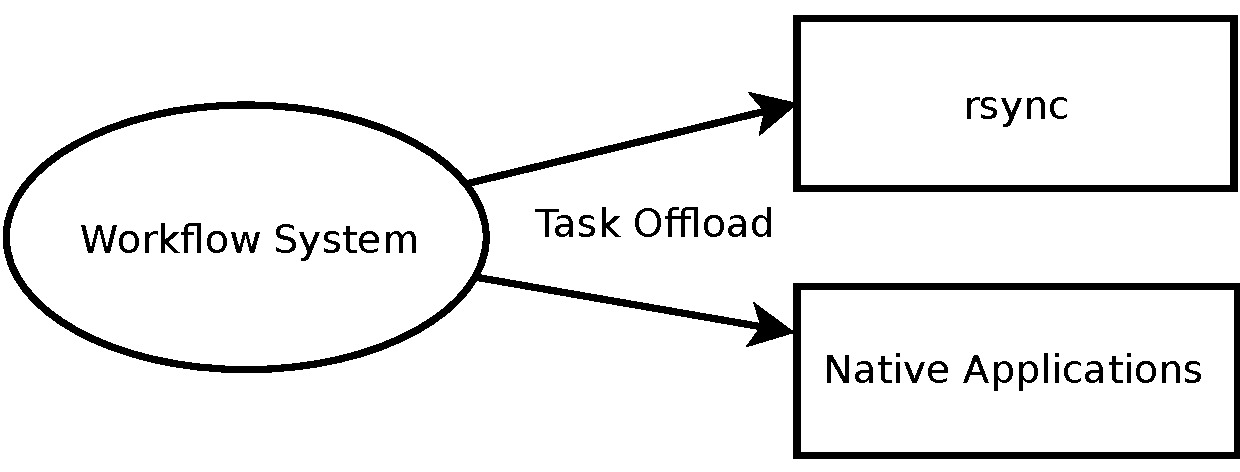
\includegraphics[scale=0.45]{figures/offload.pdf}
    \end{center}
    \caption{Performance: Task offload}
    \label{eval:offload}
\end{figure}

Due to this, a performance evaluation of the system was not deemed necessary.
Performance of the system could, however, be affected by several processes being
executed simultaneously. In order to speed up the process in this case the
system would need to be distributed to include multiple processing servers; this
was decided outside the scope of the project.

\section{Summary}

The system was evaluated and it was determined that: \begin{inparaenum}[(i)] \item
it can successfully integrate a portion of the Zamani Workflow; and \item user could
successfully use the system with very little effort.\end{inparaenum} The terminology was found
to be somewhat confusing and it was found that better filer filtering options would be
beneficial. Overall, however, the system was evaluated as being a success.

